\documentclass{beamer}

% Presentation Theme and Settings
%\usetheme{Madrid}
%\usepackage{graphicx}
%\usepackage{booktabs}

% Title Information
\title[Currency Risk Analysis]{Which of the G10 Currencies is the Riskiest to Hold for a Swiss Resident?}
\author{Yudi, Tane, Migjen}
\date{December 11, 2024}

\begin{document}

% Title Slide
\begin{frame}
  \titlepage
\end{frame}



% Table of Contents
\begin{frame}{Outline}
  \tableofcontents
\end{frame}

% Introduction Slide
\section{Introduction}
\begin{frame}{Introduction}
  \begin{itemize}
    \item Exchange rate risk is crucial for Swiss investors with foreign currency exposure.
    \item Switzerland's economy heavily relies on international trade and finance, amplifying the importance of managing exchange rate risks.
    \item G10 currencies include AUD, CAD, EUR, GBP, JPY, NOK, NZD, SEK, and USD, which are among the most traded and economically significant globally.
    \item Risks are assessed through:
    \begin{itemize}
      \item \textbf{Depreciation}
      \item \textbf{Volatility}
      \item \textbf{Maximum Drawdown} 
      \item \textbf{Value at Risk (VaR)}
    \end{itemize}
    \item This comprehensive approach ensures insights into both long-term trends and short-term risks, aiding informed decision-making for investors.
  \end{itemize}
\end{frame}



% Methodology Slide
\section{Methodology}
\begin{frame}{Methodology}
  \begin{itemize}
    \item \textbf{Data Collection:} Daily exchange rates for G10 currencies relative to CHF (2000--2024) were sourced from Investing.com. 
    \item \textbf{Metric Selection:}
    \begin{itemize}
     \item \textbf{Depreciation:} Long-term value loss against CHF, indicating structural weaknesses.
      \item \textbf{Volatility:} Fluctuations in value, reflecting uncertainty and potential instability.
      \item \textbf{Maximum Drawdown:} Worst-case declines, highlighting potential historical losses.
      \item \textbf{Value at Risk (VaR):} Statistical measure of potential losses under normal conditions.
    \end{itemize}
    \item \textbf{Rationale for Methodology:}
    \begin{itemize}
      \item The combination of metrics allows a multidimensional risk assessment.
      \item Metrics like VaR and Drawdown were selected to align with practical risk management practices used by financial institutions.
    \end{itemize}
  \end{itemize}
\end{frame}

% Analysis Slides
\section{Analysis}
\begin{frame}{Pre-Global Financial Crisis (2000--2007)}
  \begin{itemize}
    \item Depreciation:
    \begin{itemize}
      \item JPY and USD experienced significant losses.
      \item EUR showed stability and slight appreciation.
    \end{itemize}
   \end{itemize}

    \begin{figure}
    \centering
        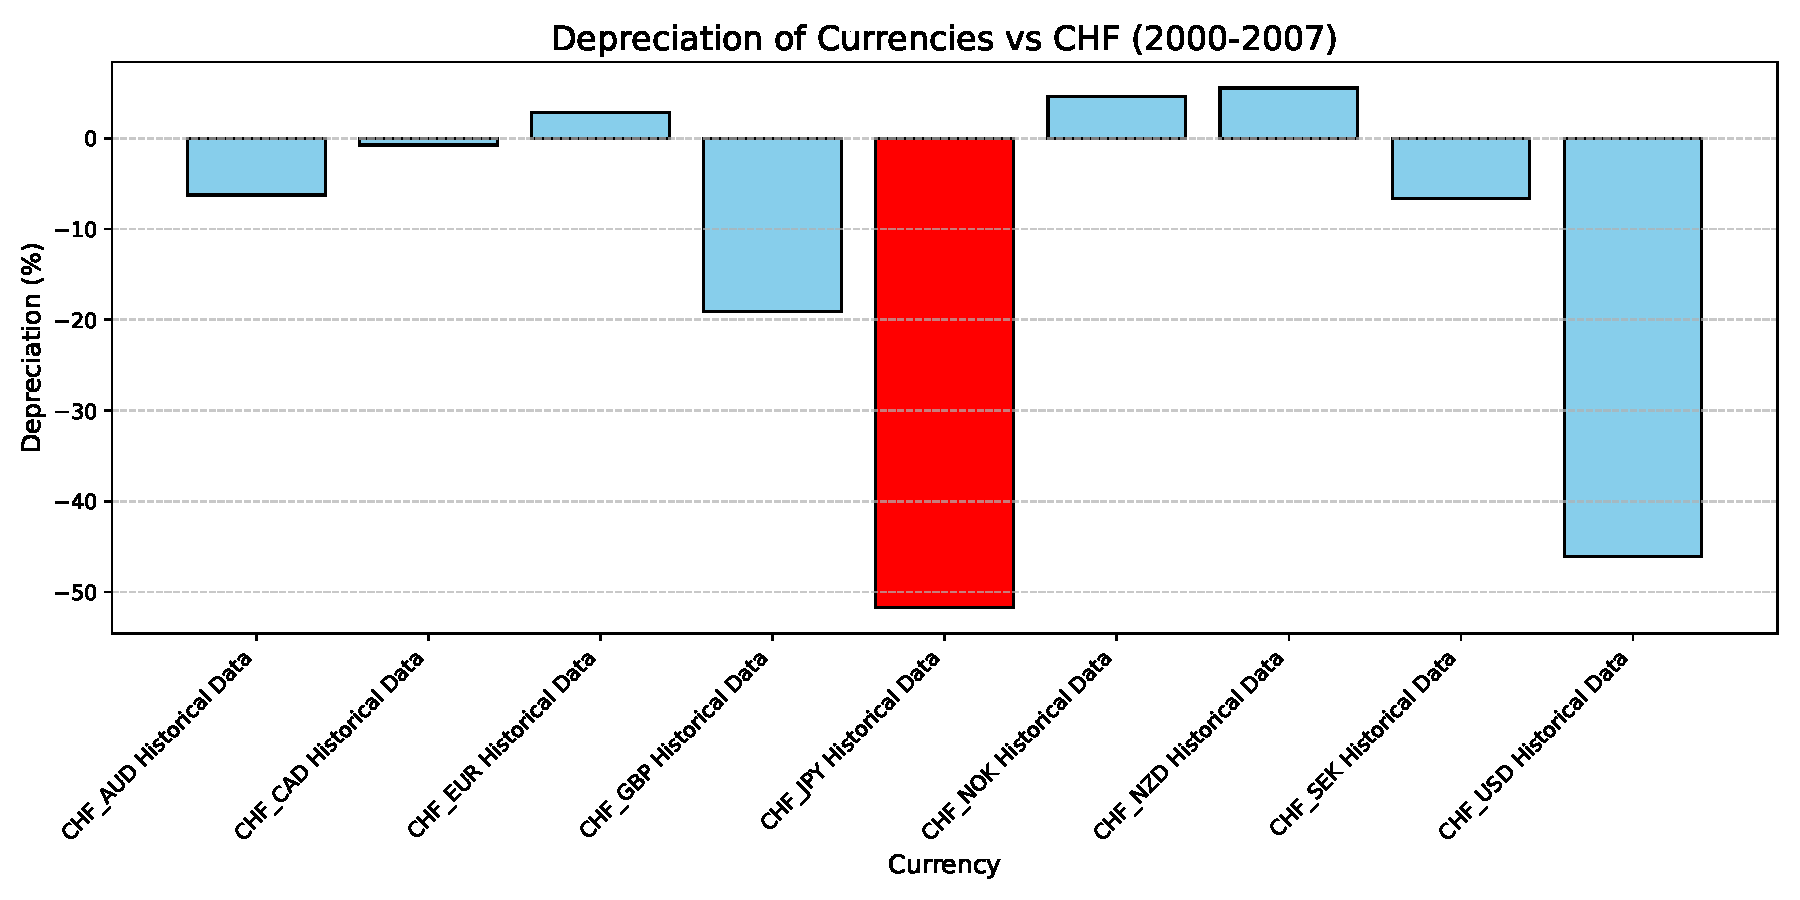
\includegraphics[width=0.75
        \textwidth]{../../images/depreciation_2000_2007.pdf}
        \caption{Depreciation of Currencies vs CHF (2000--2007).}
        \label{fig:question}
    \end{figure}
    
\end{frame}


\begin{frame}{Pre-Global Financial Crisis (2000--2007)}
  \begin{itemize}
     \item Volatility:
    \begin{itemize}
      \item AUD was the most volatile, linked to commodity exports.
    \end{itemize}
   \end{itemize}

    \begin{figure}
    \centering
        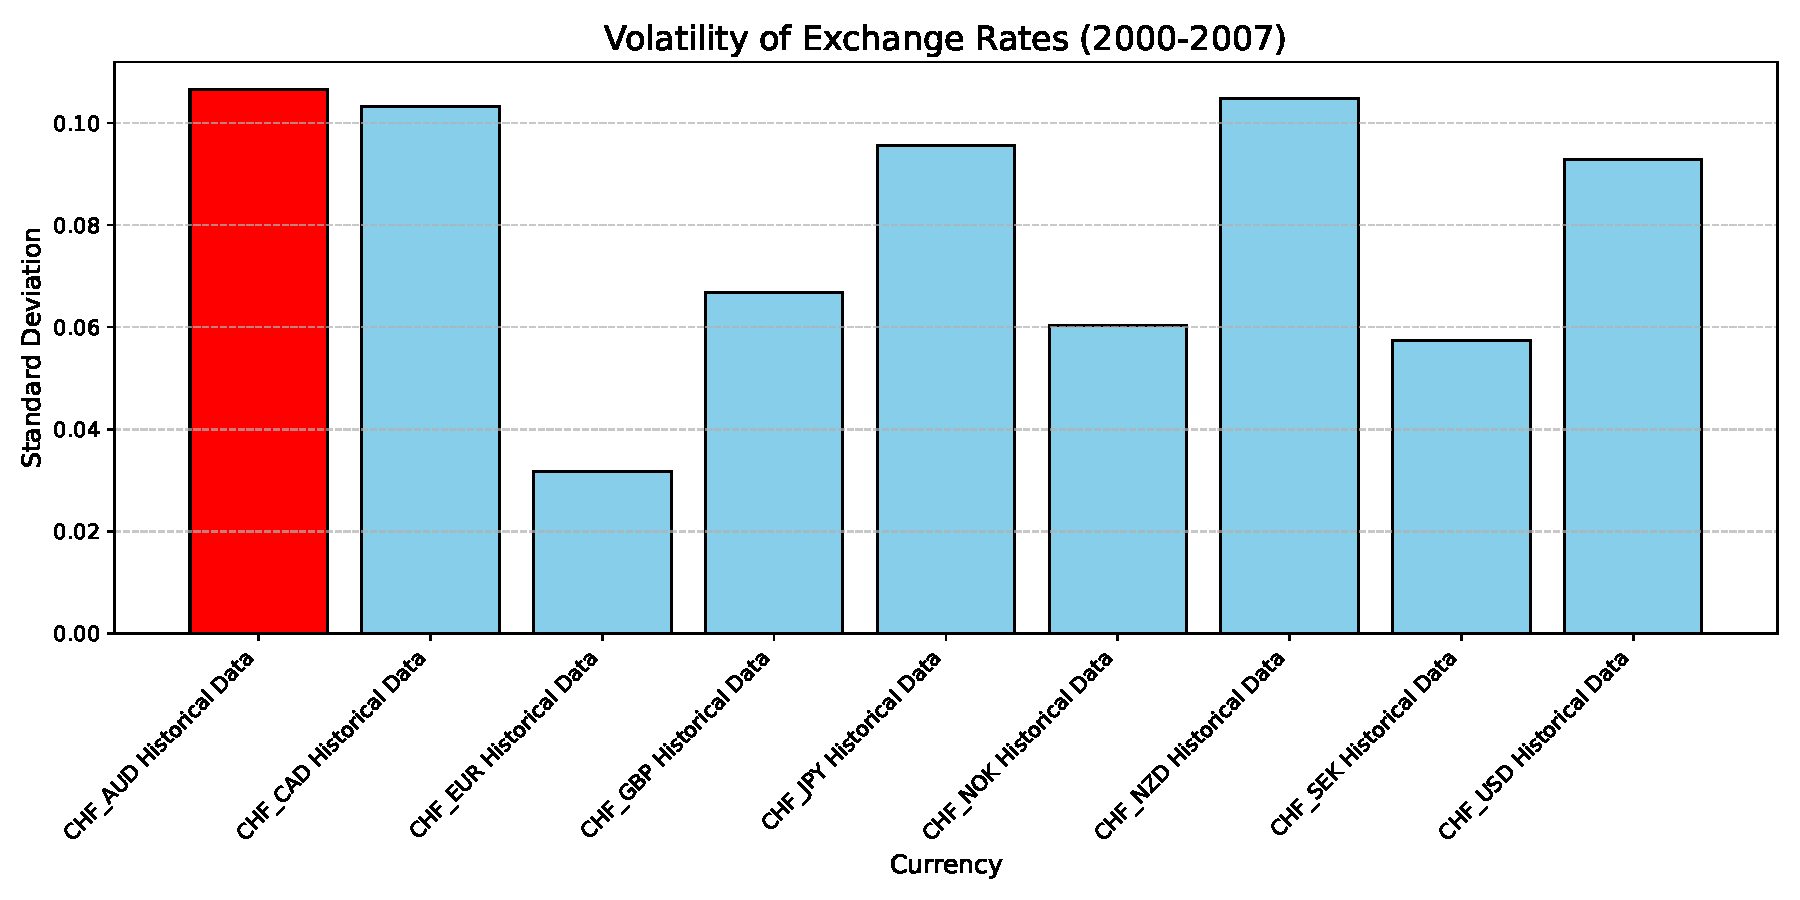
\includegraphics[width=0.75
        \textwidth]{../../images/volatility_2000_2007.pdf}
        \caption{Volatility of Exchange rates (2000--2007).}
        \label{fig:question}
    \end{figure}
    
\end{frame}


\begin{frame}{Pre-Global Financial Crisis (2000--2007)}
  \begin{itemize}
    \item Maximum Drawdown:
    \begin{itemize}
      \item Significant for JPY and USD.
    \end{itemize}
   \end{itemize}

    \begin{figure}
    \centering
        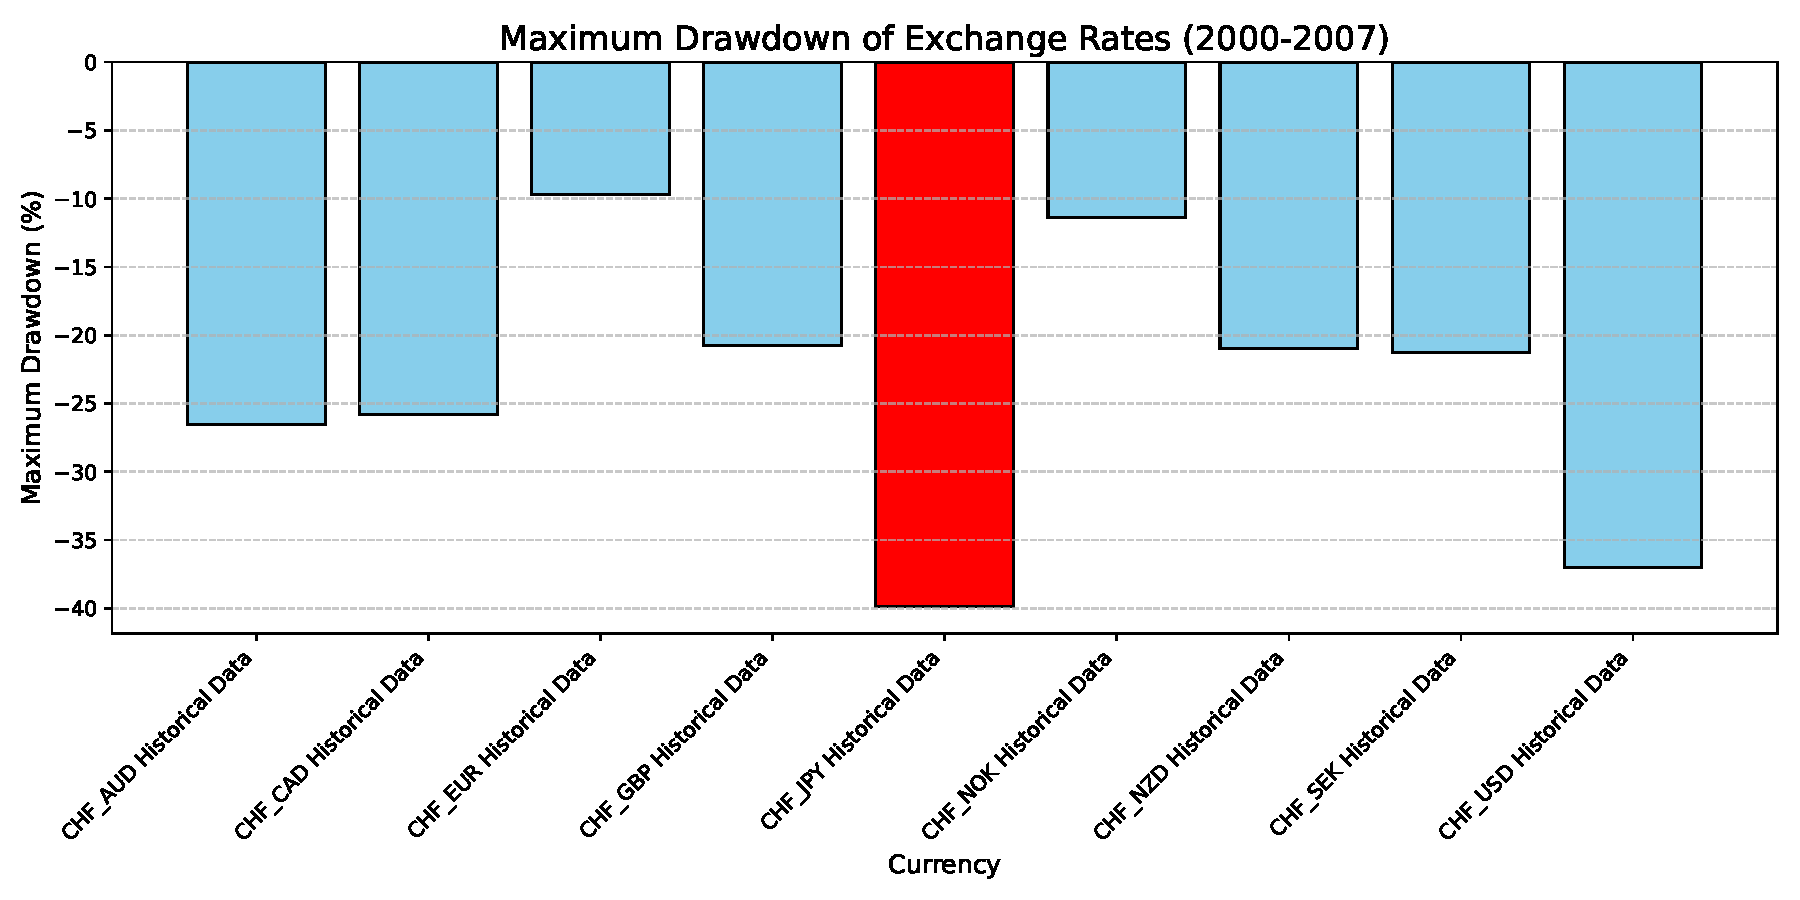
\includegraphics[width=0.75
        \textwidth]{../../images/maximum_drawdown_2000_2007.pdf}
        \caption{Maximum Drawdown of Exchange rates (2000--2007).}
        \label{fig:question}
    \end{figure}
\end{frame}

\begin{frame}{Pre-Global Financial Crisis (2000--2007)}
  \begin{itemize}
    \item Value at Risk:
    \begin{itemize}
      \item The Euro stands out as the least risky currency but Canadian Dollar displayed higher VaR levels due to its heavy reliance on energy exports.
    \end{itemize}
   \end{itemize}

    \begin{figure}[h!]
    \centering
    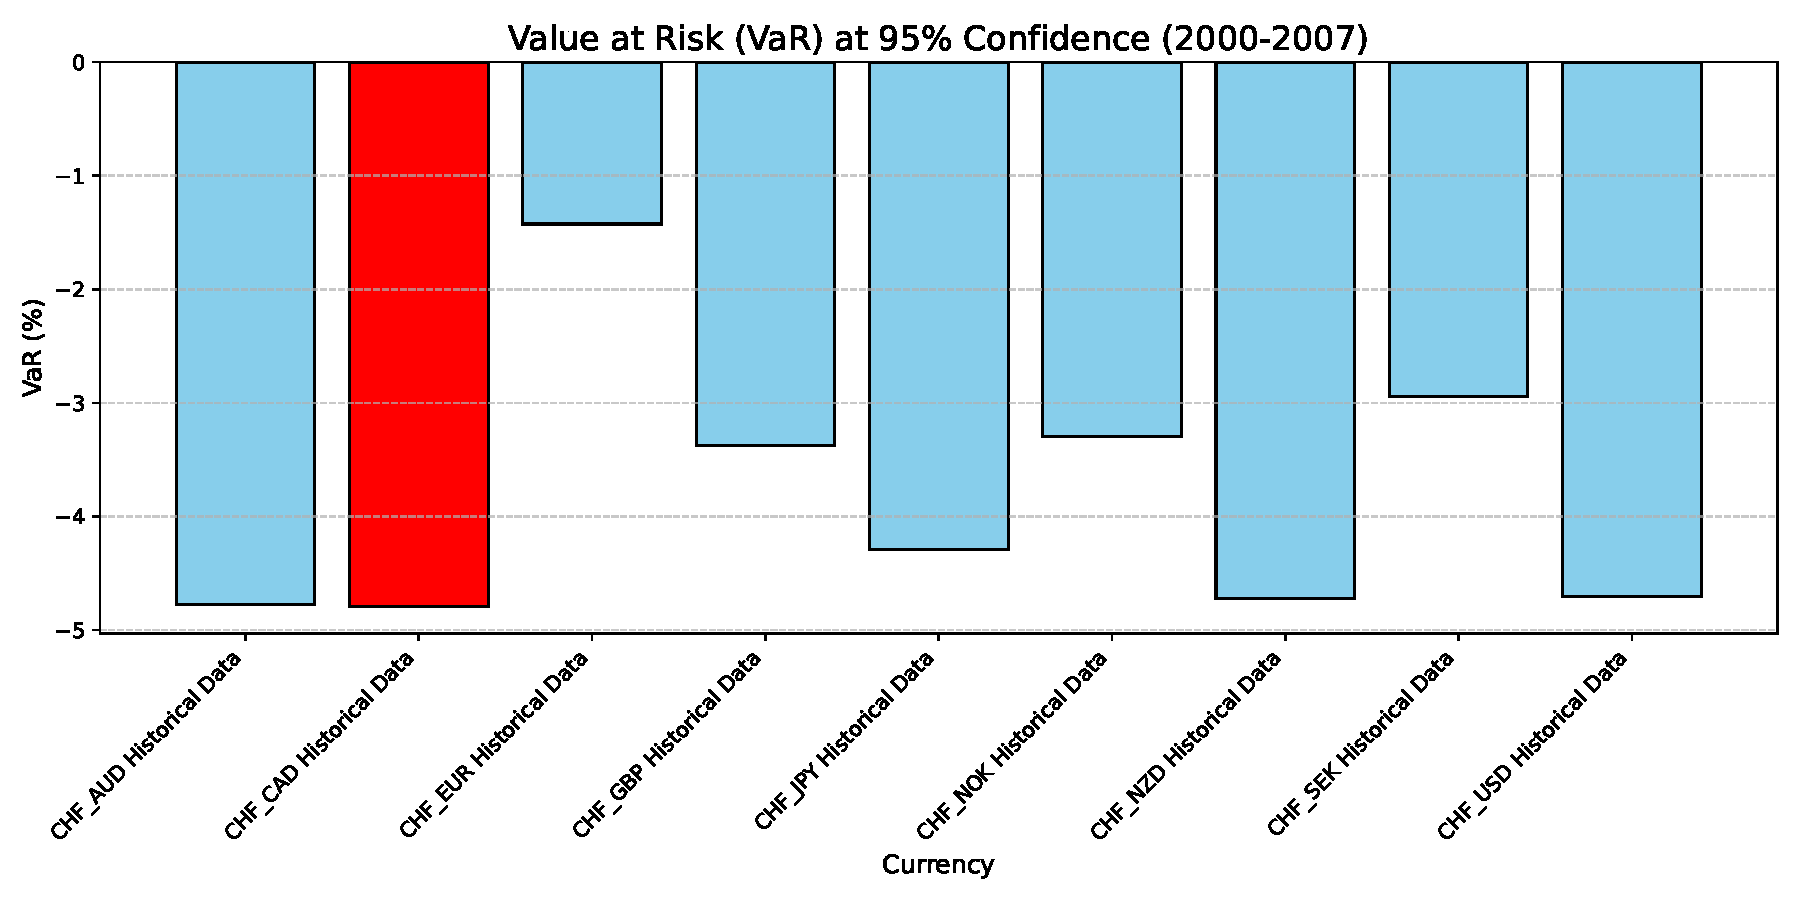
\includegraphics[width=0.75\textwidth]{../../images/var_2000_2007.pdf}
    \caption{Value at Risk of Exchange rates (2000--2007).}
    \label{fig:var_2000_2007}
\end{figure}
    
\end{frame}

\begin{frame}{During the Global Financial Crisis (2007--2009)}
  \begin{itemize}
    \item Depreciation:
    \begin{itemize}
      \item GBP faced the largest depreciation (-46\%).
    \end{itemize}
   \end{itemize}

    \begin{figure}
    \centering
        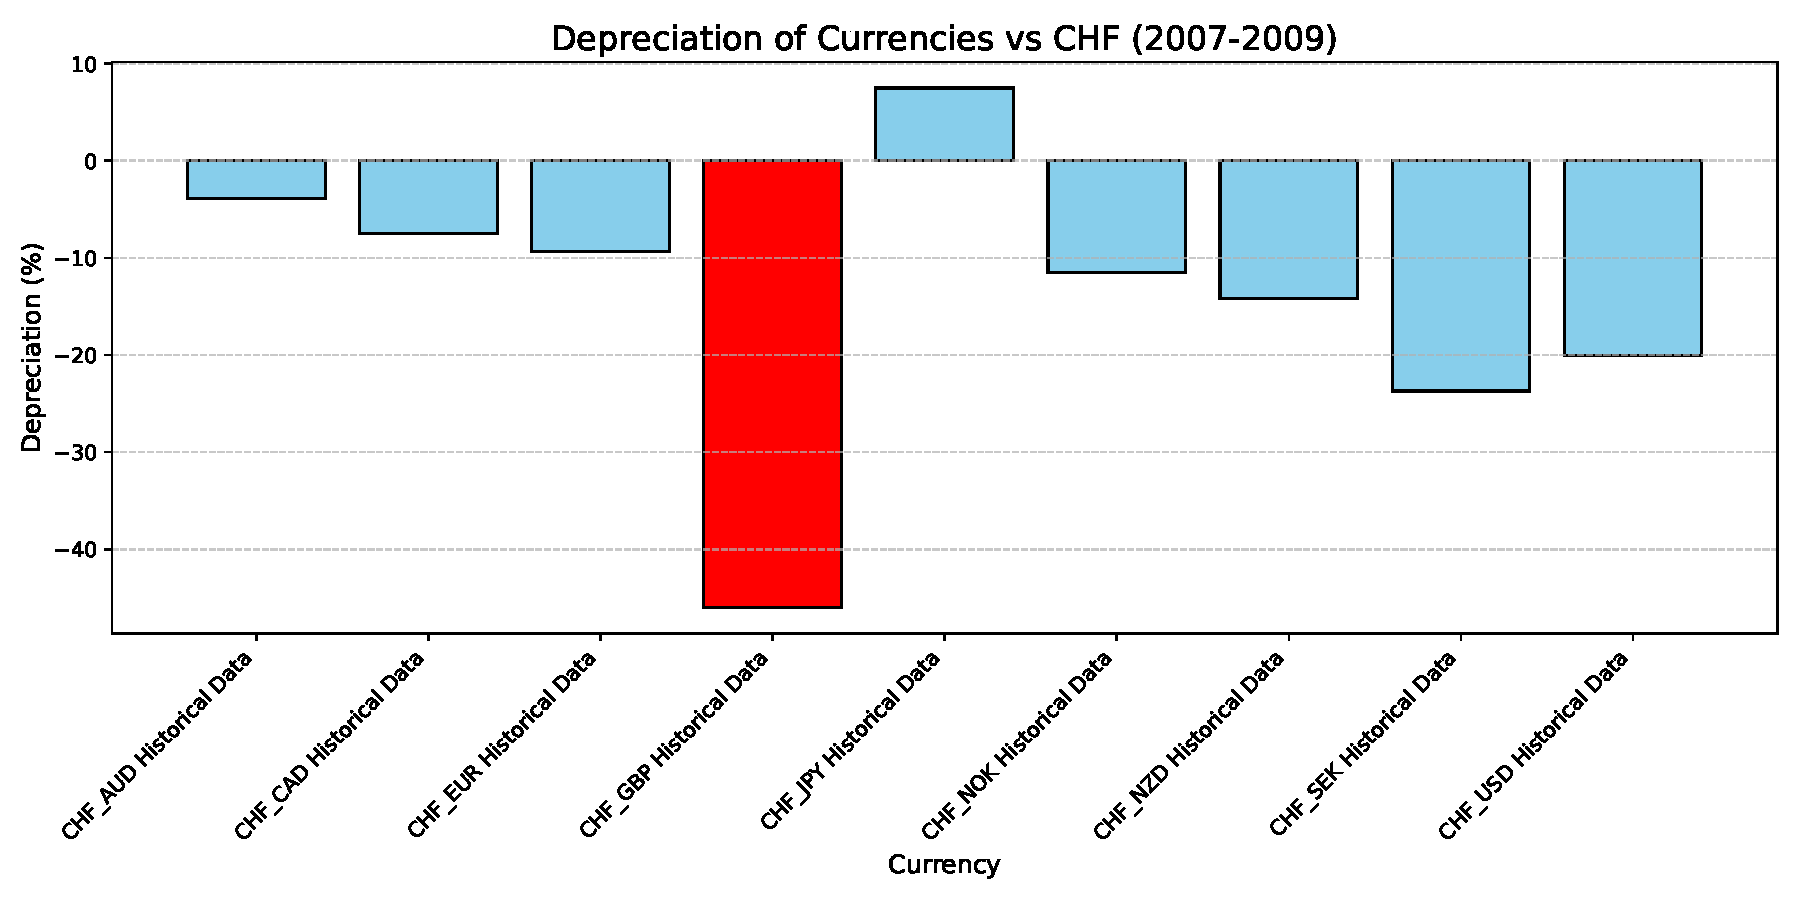
\includegraphics[width=0.75
        \textwidth]{../../images/depreciation_2007_2009.pdf}
        \caption{Depreciation of Currencies vs CHF (2007--2009).}
        \label{fig:question}
    \end{figure}
    
\end{frame}


\begin{frame}{During the Global Financial Crisis (2007--2009)}
  \begin{itemize}
     \item Volatility:
    \begin{itemize}
      \item Volatility peaked for CAD and AUD due to commodity price shocks.
    \end{itemize}
   \end{itemize}

    \begin{figure}
    \centering
        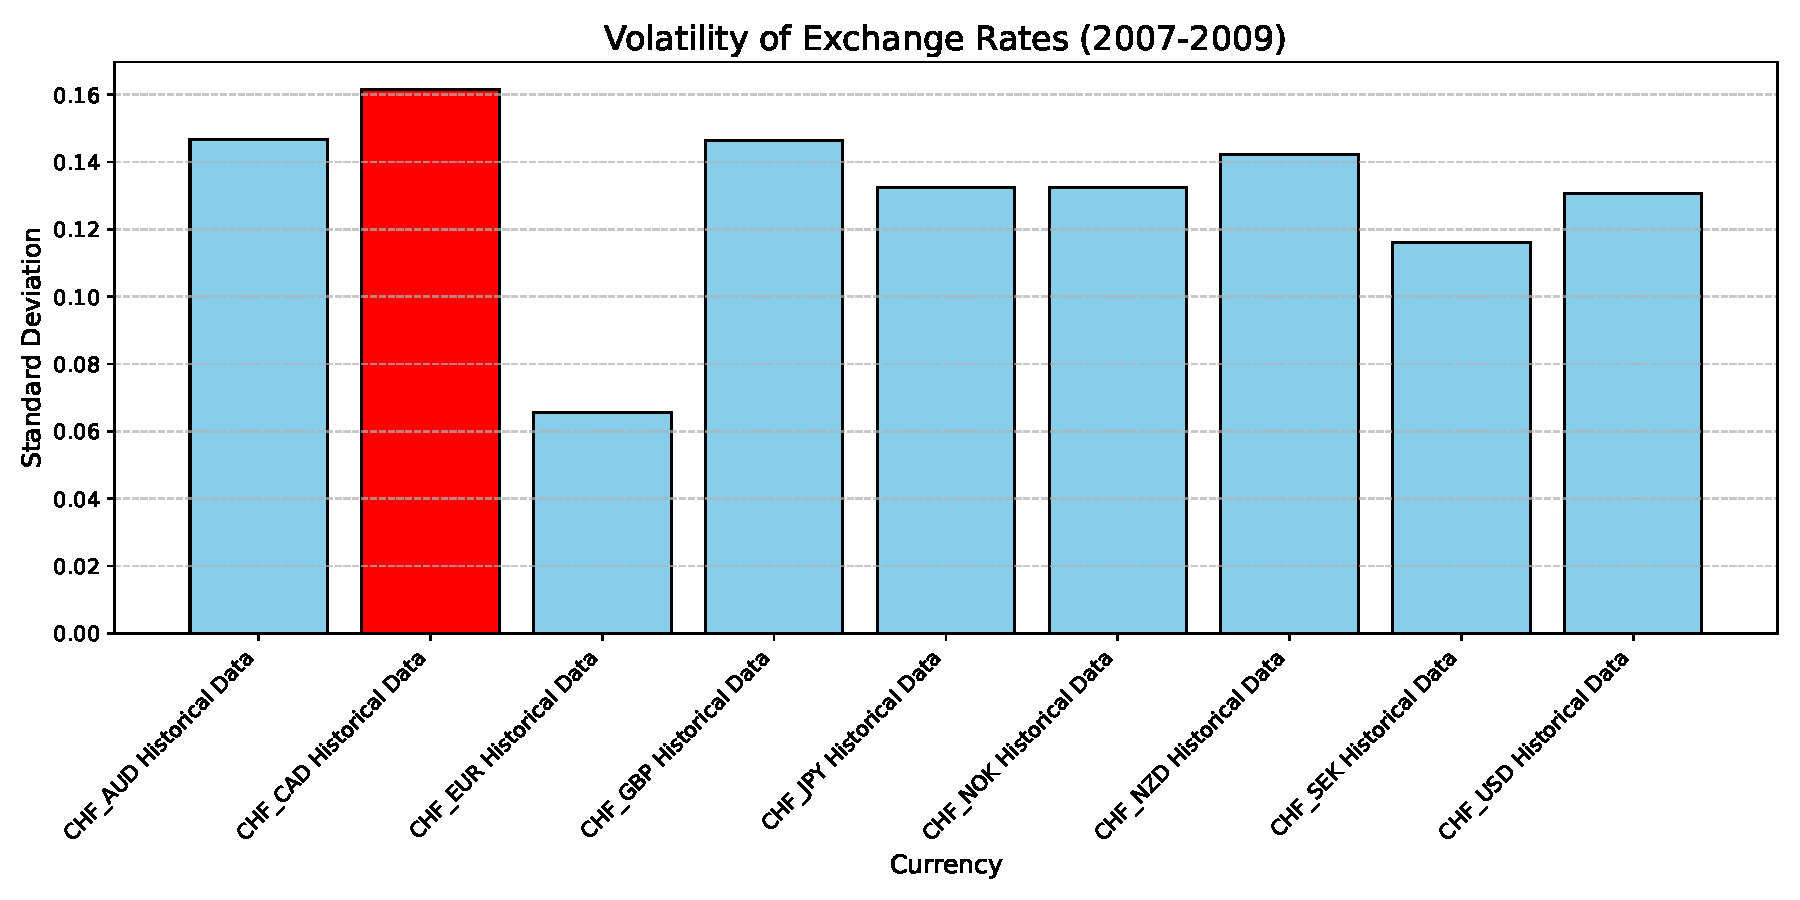
\includegraphics[width=0.75
        \textwidth]{../../images/volatility_2007_2009.pdf}
        \caption{Volatility of Exchange rates (2007--2009).}
        \label{fig:question}
    \end{figure}
    
\end{frame}


\begin{frame}{During the Global Financial Crisis (2007--2009)}
  \begin{itemize}
    \item Maximum Drawdown:
    \begin{itemize}
      \item NZD experienced the largest drawdown while Euro had
the smallest.
    \end{itemize}
   \end{itemize}

    \begin{figure}
    \centering
        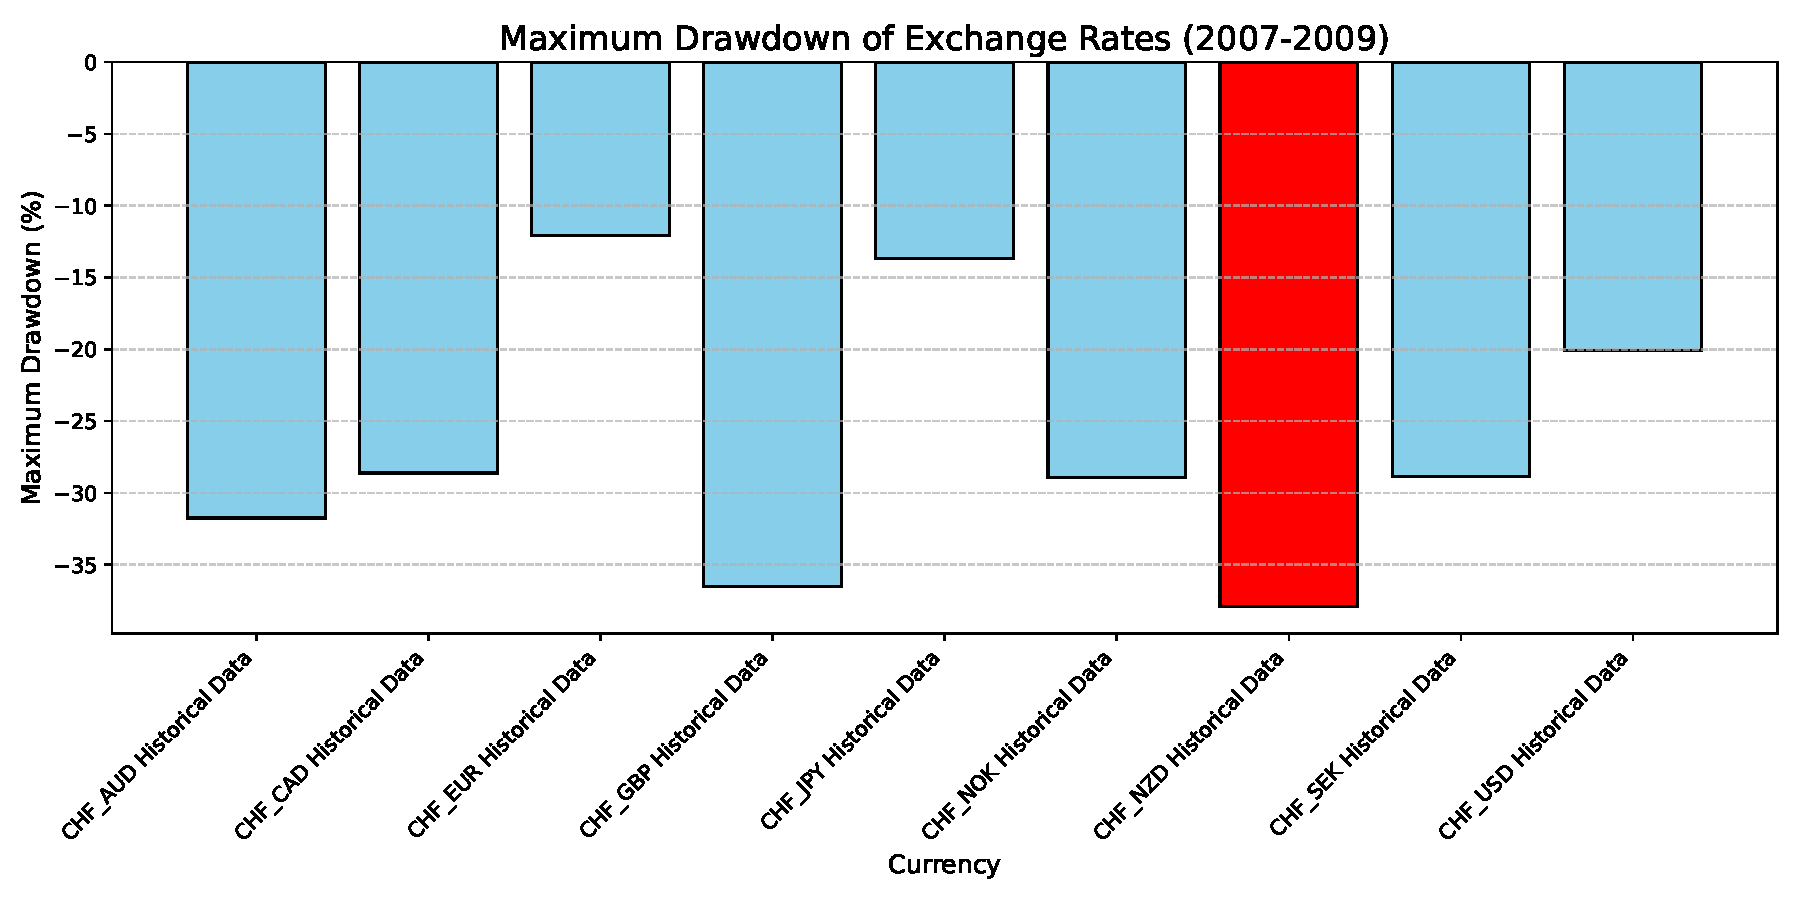
\includegraphics[width=0.75
        \textwidth]{../../images/maximum_drawdown_2007_2009.pdf}
        \caption{Maximum Drawdown of Exchange rates (2007--2009).}
        \label{fig:question}
    \end{figure}
    
\end{frame}

\begin{frame}{During the Global Financial Crisis (2007--2009)}
  \begin{itemize}
    \item Value at Risk:
    \begin{itemize}
      \item Canadian Dollar (CAD) and Australian Dollar (AUD) as the riskiest currencies, reflecting their sensitivity to commodity price shocks.
      \item Euro (EUR) demonstrated the lowest VaR, showcasing its relative stability
    \end{itemize}
   \end{itemize}

   \begin{figure}[h!]
    \centering
    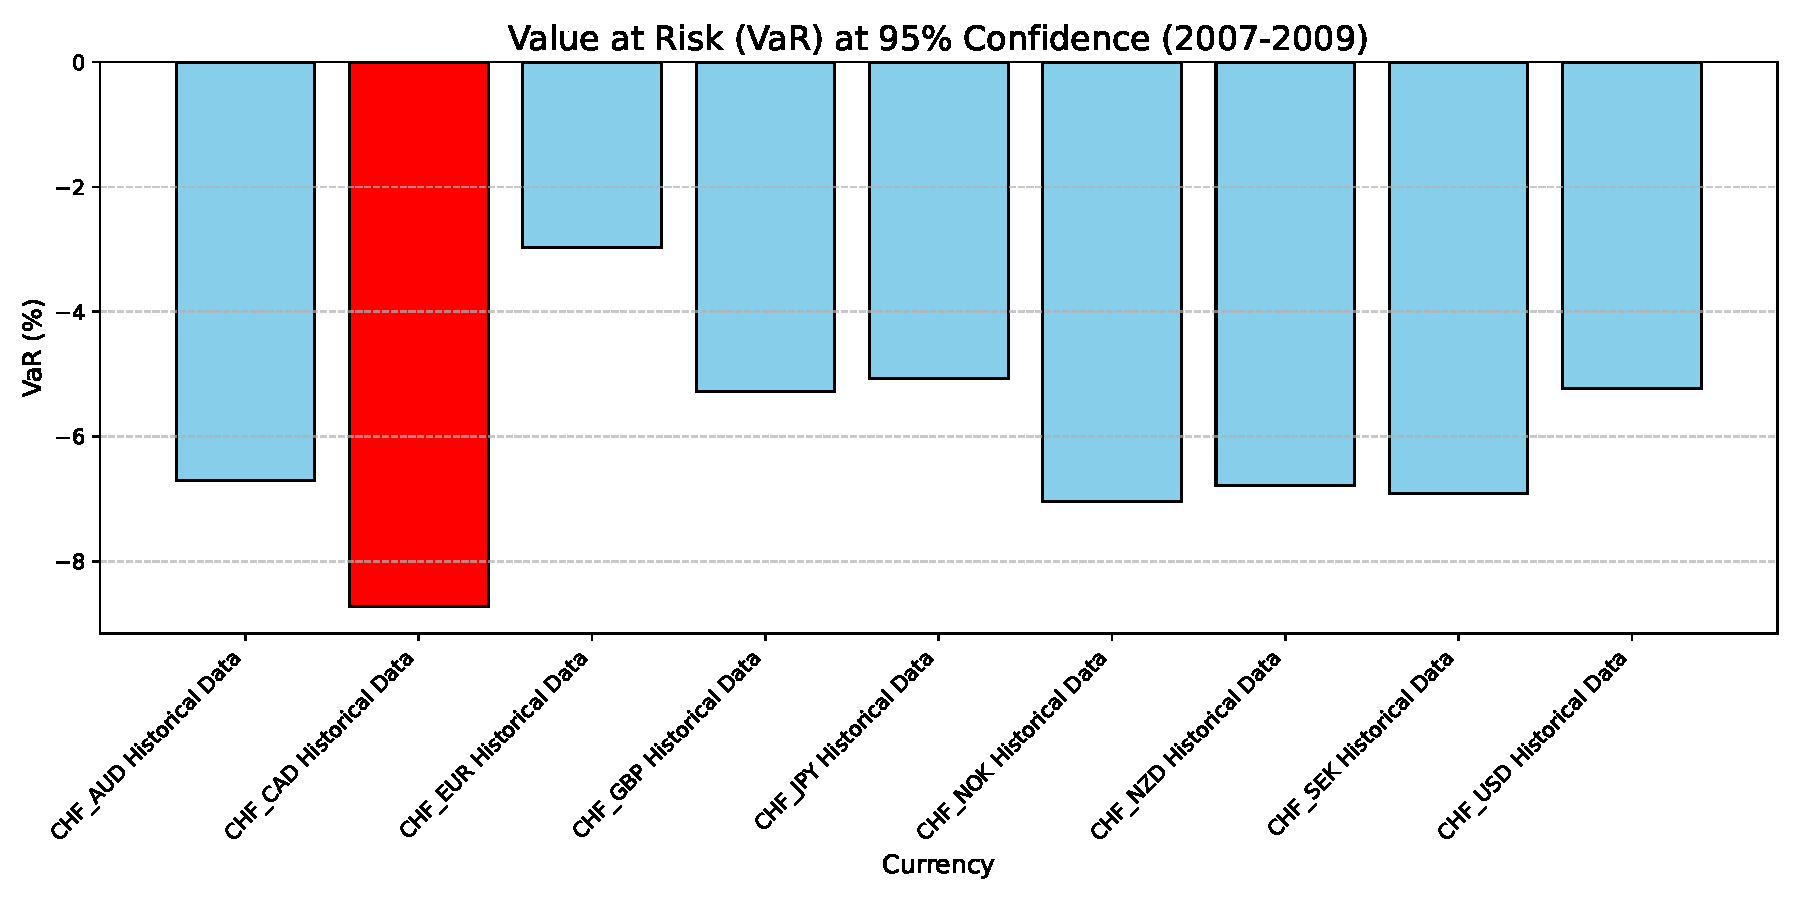
\includegraphics[width=0.75\textwidth]{../../images/var_2007_2009.pdf}
    \caption{Value at Risk of Exchange rates (2007--2009).}
    \label{fig:var_2007_2009}
\end{figure}
    
\end{frame}

\begin{frame}{Post-Financial Crisis (2009--2024)}
  \begin{itemize}
    \item Depreciation:
    \begin{itemize}
      \item JPY had the highest depreciation (-119\%).
    \end{itemize}
   \end{itemize}

   \begin{figure}[h!]
    \centering
    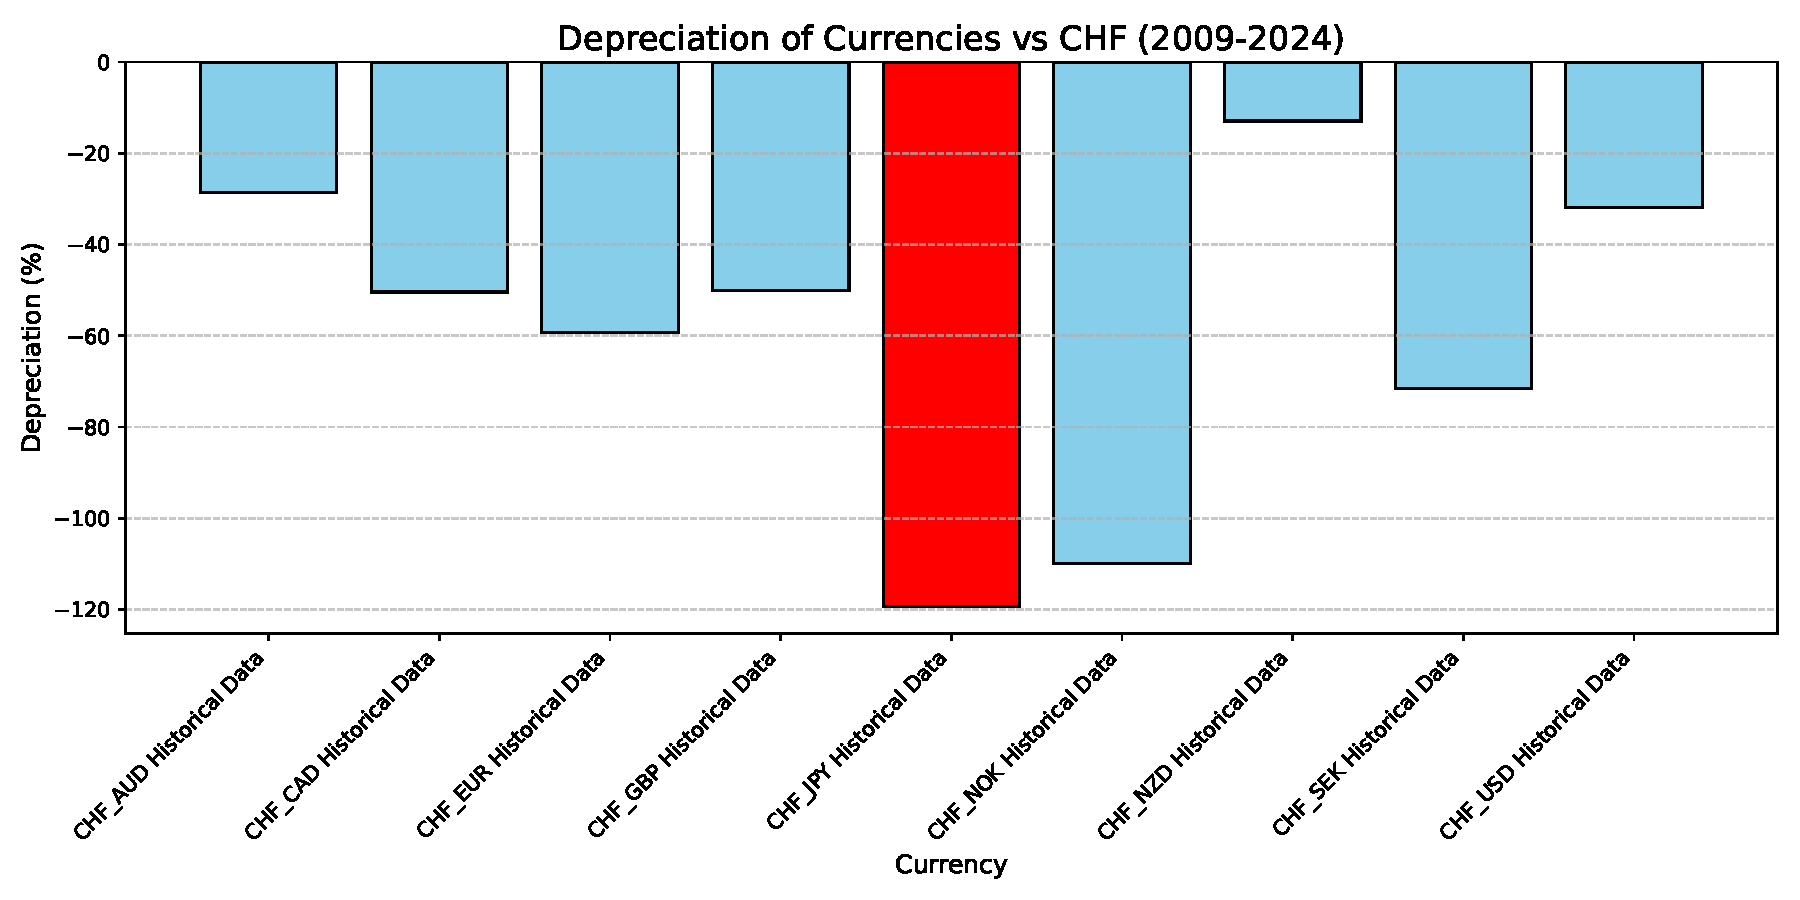
\includegraphics[width=0.75\textwidth]{../../images/depreciation_2009_2024.pdf}
    \caption{Depreciation of Currencies vs CHF (2009--2024).}
    \label{fig:depreciation_2009_2024}
\end{figure}
    
\end{frame}


\begin{frame}{Post-Financial Crisis (2009--2024)}
  \begin{itemize}
     \item Volatility:
    \begin{itemize}
      \item  New Zealand Dollar and Japanese Yen had the greatest
standard deviation values, around 0.101 and 0.100 respectively.
    \end{itemize}
   \end{itemize}

    \begin{figure}[h!]
    \centering
    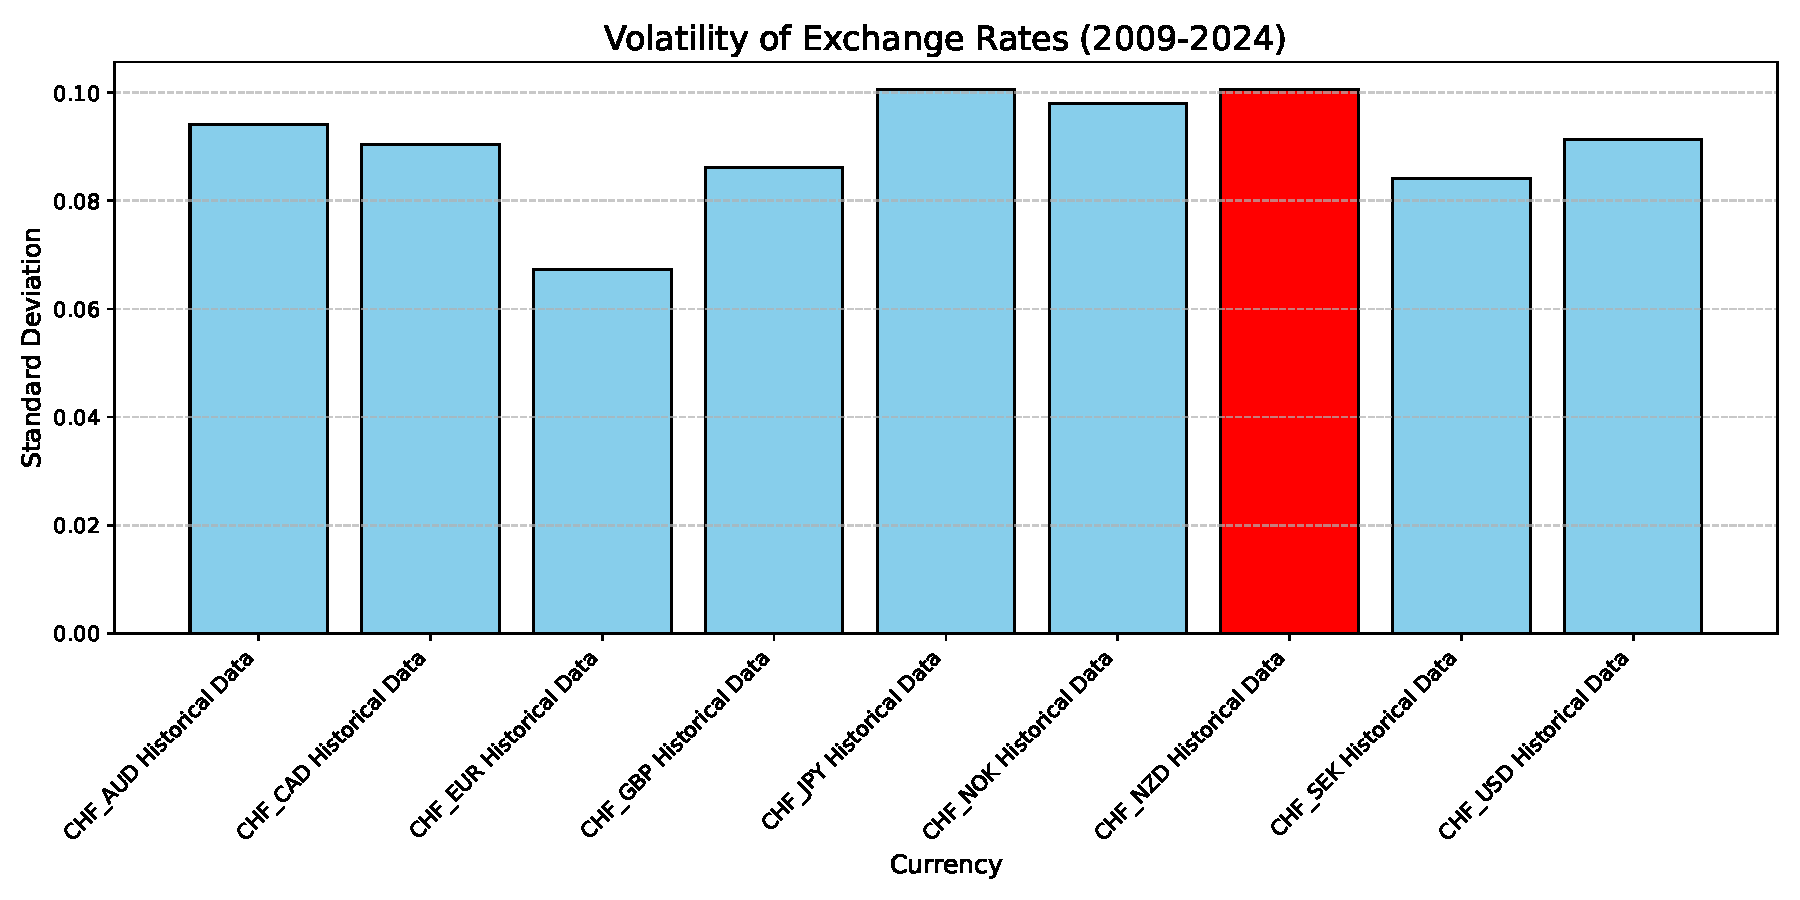
\includegraphics[width=0.75\textwidth]{../../images/volatility_2009_2024.pdf}
    \caption{Volatility of Exchange rates (2009--2024).}
    \label{fig:volatility_2009_2024}
\end{figure}
    
\end{frame}


\begin{frame}{Post-Financial Crisis (2009--2024)}
  \begin{itemize}
    \item Maximum Drawdown:
    \begin{itemize}
      \item NOK exhibited high maximum drawdown (-57\%), driven by oil price dependency.
    \end{itemize}
   \end{itemize}

   \begin{figure}[h!]
    \centering
    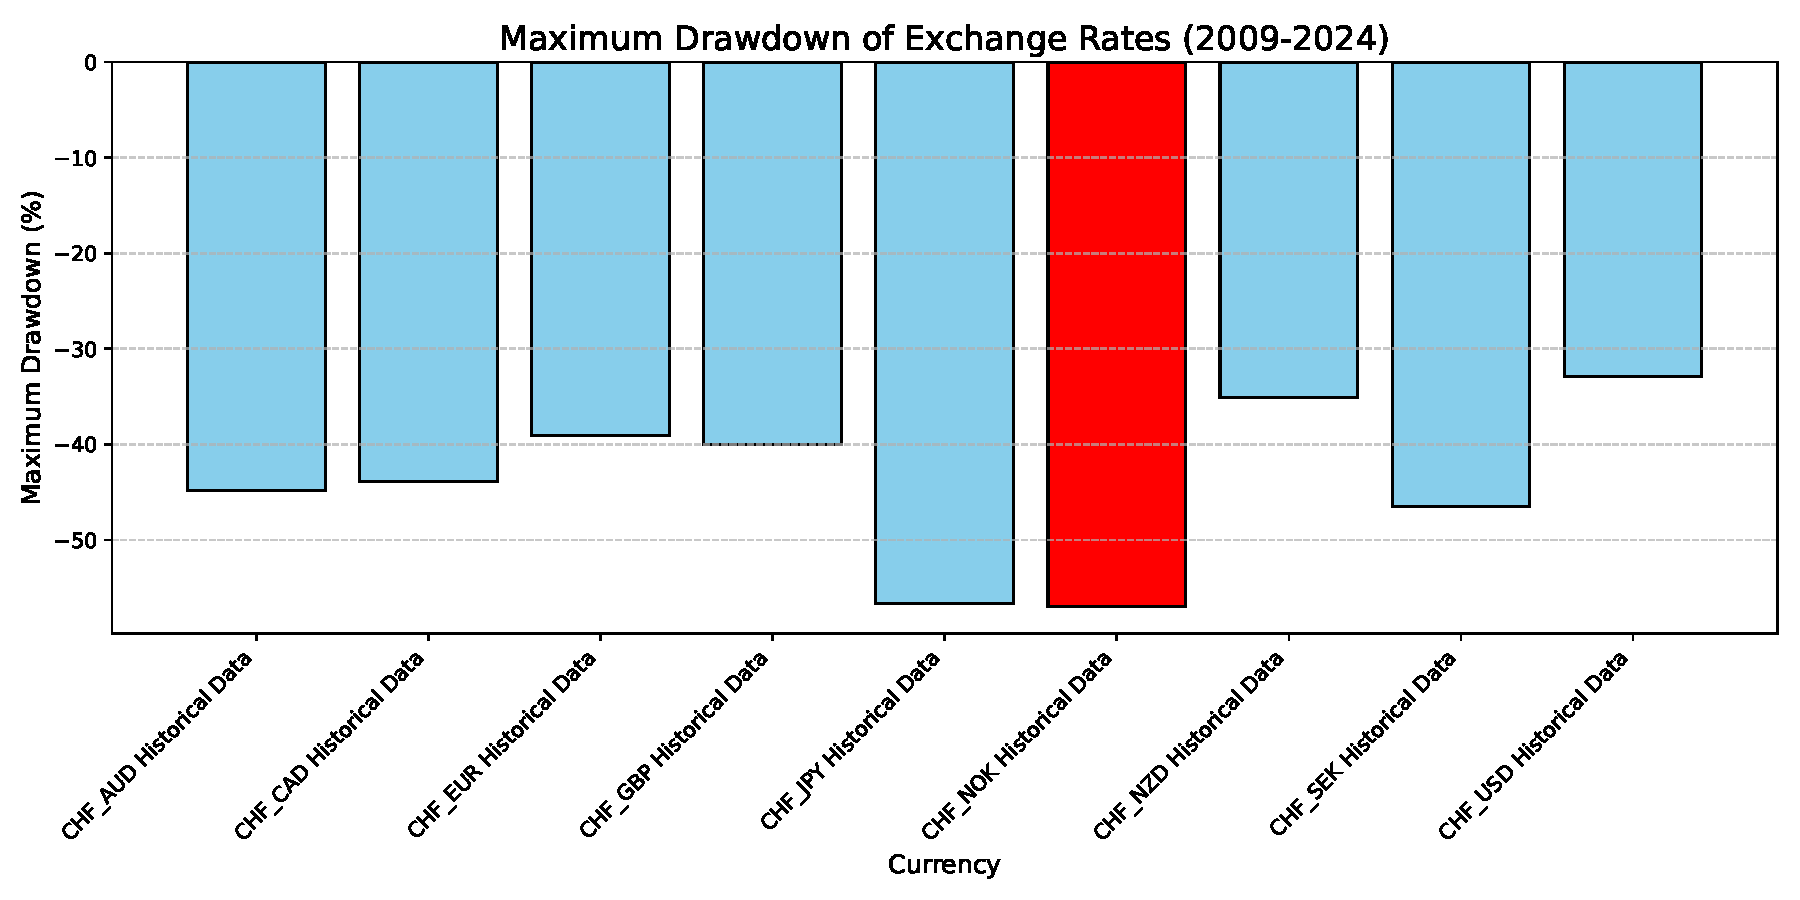
\includegraphics[width=0.75\textwidth]{../../images/maximum_drawdown_2009_2024.pdf}
    \caption{Maximum Drawdown of Exchange rates (2009--2024).}
    \label{fig:maximum_drawdown_2009_2024}
\end{figure}
    
\end{frame}

\begin{frame}{Post-Financial Crisis (2009--2024)}
  \begin{itemize}
    \item Value at Risk:
    \begin{itemize}
      \item Japanese Yen (JPY) and Norwegian Krone (NOK) exhibited the highest VaR due to speculative trading and oil price volatility.
    \end{itemize}
   \end{itemize}

   \begin{figure}[h!]
    \centering
    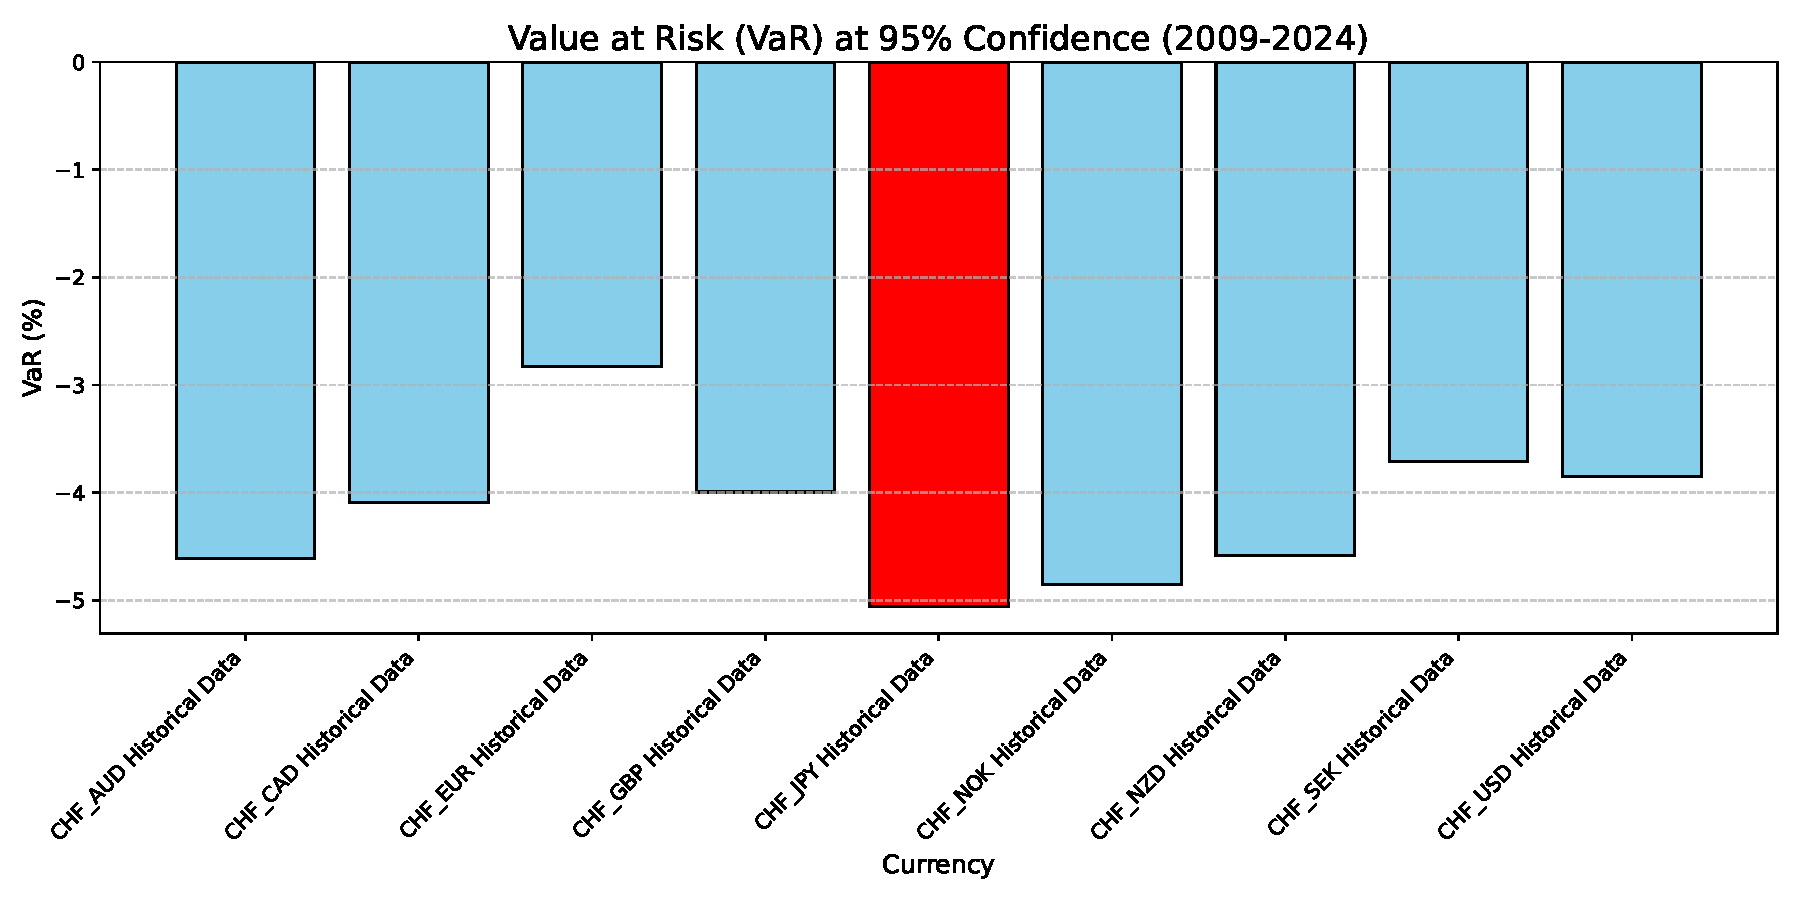
\includegraphics[width=0.75\textwidth]{../../images/var_2009_2024.pdf}
    \caption{Value at Risk of Exchange rates (2009--2024).}
    \label{fig:var_2009_2024}
\end{figure}
    
\end{frame}

\begin{frame}{Comprehensive Analysis (2000--2024)}
  \begin{itemize}
    \item JPY: Most significant depreciation (-162\%).
    \item NZD: Highest volatility (0.105).
    \item EUR: Lowest risk across all metrics.
  \end{itemize}
\end{frame}

% Conclusion Slide
\section{Conclusion}
\begin{frame}{Conclusion}
  \begin{itemize}
    \item JPY and NOK identified as the riskiest currencies for Swiss residents.
    \item EUR and CHF demonstrated stability, reflecting robust economic frameworks.
    \item Broader implications:
    \begin{itemize}
      \item Importance of diverse metrics for comprehensive risk assessment.
      \item Future work: Incorporating geopolitical and macroeconomic factors.
    \end{itemize}
  \end{itemize}
\end{frame}



\end{document}
